\documentclass{article}
\usepackage{amsmath}
\usepackage{amssymb}
\usepackage{graphicx}
\usepackage{enumitem}
\usepackage[utf8]{inputenc}
\usepackage{xcolor}

\graphicspath{{/home/stephanie/Escritorio/THC/Taller-de-Herramientas-Computacionales/Clases/Latex/Imagenes/}}

\title{\Huge Taller de Herramientas Computacionales}
\author{Stephanie Escobar Sánchez}
\date{23/enero/2019}


\begin{document}
	\maketitle
	\begin{center}
		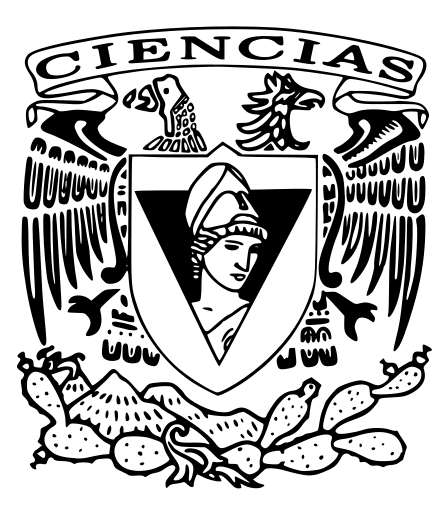
\includegraphics[scale=0.40]{1.png}	
	\end{center}
	\newpage
	\begin{center}
		\title {\textcolor{green}{\Huge \textbf{Cuestionario clase 13}} }  
	\end{center}
\textbf{¿De qué forma se puede representar una matriz sin el comando matix?}\\
Como una lista de listas\\
\\
\textbf{¿Cuál es la mejor forma de resolver los problemas?}\\
Por partes, primero lo más básico y después cosas más complejas\\
\\
\textbf{¿Qué es una función recursiva?}\\
Una función que se llama a sí misma\\
\\
\textbf{¿Cuáles son los dos elementos de las funciones recursivas?}\\
Se componen de dos elementos: bases recursivas y regla de recursividad\\
\\
\textbf{¿Cómo se llama a las funciones recursivas?}\\
Como procedimientos y subrutinas\\
\\
\textbf{¿Qué es el ámbito de validez}\\
Es dónde son visibles las variables\\
\\
\textbf{¿Por qué es importante etiquetar explícitamente las variables?}\\
Para evitar confusiones.
\end{document}